% Options for packages loaded elsewhere
\PassOptionsToPackage{unicode}{hyperref}
\PassOptionsToPackage{hyphens}{url}
\documentclass[
]{website}
\usepackage{xcolor}
\usepackage{amsmath,amssymb}
\setcounter{secnumdepth}{5}
\usepackage{iftex}
\ifPDFTeX
  \usepackage[T1]{fontenc}
  \usepackage[utf8]{inputenc}
  \usepackage{textcomp} % provide euro and other symbols
\else % if luatex or xetex
  \usepackage{unicode-math} % this also loads fontspec
  \defaultfontfeatures{Scale=MatchLowercase}
  \defaultfontfeatures[\rmfamily]{Ligatures=TeX,Scale=1}
\fi
\usepackage{lmodern}
\ifPDFTeX\else
  % xetex/luatex font selection
\fi
% Use upquote if available, for straight quotes in verbatim environments
\IfFileExists{upquote.sty}{\usepackage{upquote}}{}
\IfFileExists{microtype.sty}{% use microtype if available
  \usepackage[]{microtype}
  \UseMicrotypeSet[protrusion]{basicmath} % disable protrusion for tt fonts
}{}
\makeatletter
\@ifundefined{KOMAClassName}{% if non-KOMA class
  \IfFileExists{parskip.sty}{%
    \usepackage{parskip}
  }{% else
    \setlength{\parindent}{0pt}
    \setlength{\parskip}{6pt plus 2pt minus 1pt}}
}{% if KOMA class
  \KOMAoptions{parskip=half}}
\makeatother
\usepackage{longtable,booktabs,array}
\usepackage{calc} % for calculating minipage widths
% Correct order of tables after \paragraph or \subparagraph
\usepackage{etoolbox}
\makeatletter
\patchcmd\longtable{\par}{\if@noskipsec\mbox{}\fi\par}{}{}
\makeatother
% Allow footnotes in longtable head/foot
\IfFileExists{footnotehyper.sty}{\usepackage{footnotehyper}}{\usepackage{footnote}}
\makesavenoteenv{longtable}
\usepackage{graphicx}
\makeatletter
\newsavebox\pandoc@box
\newcommand*\pandocbounded[1]{% scales image to fit in text height/width
  \sbox\pandoc@box{#1}%
  \Gscale@div\@tempa{\textheight}{\dimexpr\ht\pandoc@box+\dp\pandoc@box\relax}%
  \Gscale@div\@tempb{\linewidth}{\wd\pandoc@box}%
  \ifdim\@tempb\p@<\@tempa\p@\let\@tempa\@tempb\fi% select the smaller of both
  \ifdim\@tempa\p@<\p@\scalebox{\@tempa}{\usebox\pandoc@box}%
  \else\usebox{\pandoc@box}%
  \fi%
}
% Set default figure placement to htbp
\def\fps@figure{htbp}
\makeatother
\setlength{\emergencystretch}{3em} % prevent overfull lines
\providecommand{\tightlist}{%
  \setlength{\itemsep}{0pt}\setlength{\parskip}{0pt}}
\usepackage[]{natbib}
\bibliographystyle{plainnat}
\usepackage{booktabs}
\usepackage{bookmark}
\IfFileExists{xurl.sty}{\usepackage{xurl}}{} % add URL line breaks if available
\urlstyle{same}
\hypersetup{
  pdftitle={Resumen del Tema 1 de Psicología Social},
  pdfauthor={David Alarcón},
  hidelinks,
  pdfcreator={LaTeX via pandoc}}

\title{Resumen del Tema 1 de Psicología Social}
\author{David Alarcón}
\date{2024-10-17}

\begin{document}
\maketitle

{
\setcounter{tocdepth}{2}
\tableofcontents
}
\section*{Psicología Social}\label{book}
\addcontentsline{toc}{section}{Psicología Social}

\emph{Este resumen del tema es sólo para uso como material de apoyo en las tutorías. Para estudiar y preparar el examén se recomienda usar el libro referenciado en la guía de la asignatura.}

\section*{Tema 1: Introducción a la psicología social}\label{tema-1-introducciuxf3n-a-la-psicologuxeda-social}
\addcontentsline{toc}{section}{Tema 1: Introducción a la psicología social}

\subsection*{\texorpdfstring{\hyperref[tema1]{1. ¿Qué es la Psicología Social y qué hace?}}{1. ¿Qué es la Psicología Social y qué hace?}}\label{quuxe9-es-la-psicologuxeda-social-y-quuxe9-hace}
\addcontentsline{toc}{subsection}{\hyperref[tema1]{1. ¿Qué es la Psicología Social y qué hace?}}

\begin{itemize}
\tightlist
\item
  \hyperref[subtema1_1]{1.1 La Psicología Social es una disciplina científica}
\item
  \hyperref[subtema1_2]{1.2 La Psicología Social se centra en el comportamiento de las personas}

  \begin{itemize}
  \tightlist
  \item
    \hyperref[cuadro1_2_1]{El saludo de apertura}
  \end{itemize}
\item
  \hyperref[subtema1_3]{1.3 La Psicología Social busca comprender las causas del comportamiento social}
\item
  \hyperref[subtema1_4]{1.4 La Psicología Social busca los principios básicos en un mundo social que cambia}
\item
  \hyperref[subtema1_5]{1.5 Diferencias entre la Psicología Social y el sentido común}

  \begin{itemize}
  \tightlist
  \item
    \hyperref[subtema1_5_1]{El sesgo retrospectivo}
  \end{itemize}
\item
  \hyperref[subtema1_6]{1.6 El lugar de la Psicología Social en las Ciencias Sociales}
\end{itemize}

\subsection*{\texorpdfstring{\hyperref[tema2]{2. Principios Básicos de la Psicología Social}}{2. Principios Básicos de la Psicología Social}}\label{principios-buxe1sicos-de-la-psicologuxeda-social}
\addcontentsline{toc}{subsection}{\hyperref[tema2]{2. Principios Básicos de la Psicología Social}}

\begin{itemize}
\tightlist
\item
  \hyperref[subtema2_1]{2.1 Construimos nuestra realidad social}

  \begin{itemize}
  \tightlist
  \item
    \hyperref[cuadro2_1]{El Dilema del Prisionero}
  \end{itemize}
\item
  \hyperref[subtema2_2]{2.2 Los motivos sociales}

  \begin{itemize}
  \tightlist
  \item
    \hyperref[subtema2_2_1]{1. Pertenencia}
  \item
    \hyperref[subtema2_2_2]{2. Comprensión colectiva o compartida}
  \item
    \hyperref[subtema2_2_3]{3. Control}
  \item
    \hyperref[subtema2_2_4]{4. Perfeccionamiento de sí mismo}
  \item
    \hyperref[subtema2_2_5]{5. Confianza}
  \item
    \hyperref[subtema2_2_6]{Resumen de los motivos sociales centrales}
  \end{itemize}
\item
  \hyperref[subtema2_3]{2.3 La interconexión de los procesos psicosociales}

  \begin{itemize}
  \tightlist
  \item
    \hyperref[subtema2_3_1]{2.3.1 Críticas al reduccionismo en Psicología Social}
  \item
    \hyperref[subtema2_3_2]{2.3.2 La conexión entre los procesos psicosociales}
  \item
    \hyperref[subtema2_3_3]{2.3.3 El efecto de discontinuidad individuo-grupo}
  \end{itemize}
\item
  \hyperref[subtema2_4]{2.4 Comportamiento social y cognición social}
\item
  \hyperref[subtema2_5]{2.5 El papel de la emoción en la Psicología Social}
\item
  \hyperref[subtema2_6]{2.6 Importancia de las relaciones sociales para el bienestar de las personas}
\item
  \hyperref[subtema2_7]{2.7 La importancia de la diversidad social}
\end{itemize}

\subsection*{\texorpdfstring{\hyperref[tema3]{3. Cómo responden los psicólogos sociales a las preguntas que se plantean: la investigación en psicología social}}{3. Cómo responden los psicólogos sociales a las preguntas que se plantean: la investigación en psicología social}}\label{cuxf3mo-responden-los-psicuxf3logos-sociales-a-las-preguntas-que-se-plantean-la-investigaciuxf3n-en-psicologuxeda-social}
\addcontentsline{toc}{subsection}{\hyperref[tema3]{3. Cómo responden los psicólogos sociales a las preguntas que se plantean: la investigación en psicología social}}

\begin{itemize}
\tightlist
\item
  \hyperref[subtema3_1]{3.1 Teorías científicas: formulación y puesta a prueba de hipótesis}
\item
  \hyperref[subtema3_2]{3.2 Métodos de investigación en Psicología Social}
\item
  \hyperref[subtema3_3]{3.3. El experimento: generación del conocimiento a través de la intervención sistemática}

  \begin{itemize}
  \tightlist
  \item
    \hyperref[subtema3_3_1]{3.3.1. Control: manipulación de variables (y asignación aleatoria)}
  \item
    \hyperref[subtema3_3_2]{3.3.2. Experimentos de laboratorio}
  \item
    \hyperref[subtema3_3_3]{3.3.3. Experimentos de campo}
  \item
    \hyperref[subtema3_3_4]{3.3.4. Otras reflexiones sobre la causalidad}
  \end{itemize}
\item
  \hyperref[subtema3_4]{3.4. Métodos correlacionales}

  \begin{itemize}
  \tightlist
  \item
    \hyperref[subtema3_4_1]{3.4.1. Correlación: la búsqueda de relaciones}
  \item
    \hyperref[subtema3_4_2]{3.4.2. Investigación mediante encuestas}
  \end{itemize}
\item
  \hyperref[subtema3_5]{3.5 Observación sistemática: describir el mundo que nos rodea}
\item
  \hyperref[subtema3_6]{3.6. Investigación cualitativa y análisis del discurso}
\item
  \hyperref[subtema3_7]{3.7. Metaanálisis y revisiones sistemáticas de la literatura científica}
\item
  \hyperref[subtema3_8]{3.8. La ética en la investigación en Psicología Social}
\end{itemize}

\subsection*{\texorpdfstring{\hyperref[tema4]{4. Una breve historia de la psicología social}}{4. Una breve historia de la psicología social}}\label{una-breve-historia-de-la-psicologuxeda-social}
\addcontentsline{toc}{subsection}{\hyperref[tema4]{4. Una breve historia de la psicología social}}

\subsection*{\texorpdfstring{\hyperref[glosario1]{Glosaro Tema 1: Introducción a la psicología social}}{Glosaro Tema 1: Introducción a la psicología social}}\label{glosaro-tema-1-introducciuxf3n-a-la-psicologuxeda-social}
\addcontentsline{toc}{subsection}{\hyperref[glosario1]{Glosaro Tema 1: Introducción a la psicología social}}

\begin{center}\rule{0.5\linewidth}{0.5pt}\end{center}

\section*{1. ¿Qué es la Psicología Social y qué hace?}\label{tema1}
\addcontentsline{toc}{section}{1. ¿Qué es la Psicología Social y qué hace?}

La Psicología Social estudia cómo y por qué las personas piensan, sienten y se comportan en situaciones sociales, ya sea en presencia real, imaginaria o simbólica de otras personas.

De esta forma, investiga cómo los entornos sociales en los que nos encontramos son influenciados por otras personas o por nuestros pensamientos sobre ellas.

\subsection*{1.1 La Psicología Social es una disciplina científica}\label{subtema1_1}
\addcontentsline{toc}{subsection}{1.1 La Psicología Social es una disciplina científica}

El término ``ciencia'' alude a:

\begin{itemize}
\tightlist
\item
  La adhesión a un conjunto de valores básicos: \textbf{objetividad}
\item
  El uso de métodos para estudiar sistemáticamente cualquier faceta del mundo
\end{itemize}

Existen cuatro valores básicos que motivan la actividad científica y hacen que esta pueda ser considerada como tal:

\begin{itemize}
\tightlist
\item
  \textbf{EXACTITUD}: Adhesión del científico a una búsqueda y evaluación de la información sobre la realidad de forma rigurosa, precisa y que intenta apartarse de cualquier error.
\item
  \textbf{OBJETIVIDAD}: Conseguir y evaluar la información relativa al objeto de estudio en sí mismo, con independencia de la forma de pensar o sentir de la persona que recoge esa información.
\item
  \textbf{ESCEPTICISMO}: Los resultados se aceptan solo si han sido verificados repetidamente (replicación).
\item
  \textbf{APERTURA MENTAL}: Disposición para actualizar las conclusiones cuando haya evidencia nueva.
\end{itemize}

\subsection*{1.2 La Psicología Social se centra en el comportamiento de las personas}\label{subtema1_2}
\addcontentsline{toc}{subsection}{1.2 La Psicología Social se centra en el comportamiento de las personas}

El comportamiento de las personas es lo que estudiamos, ya que es observable y puede ser medido (por ejemplo, cuántos segundos tarda una persona en hacer una atribución de árabe-malo en comparación con árabe-bueno).

El comportamiento no se reduce únicamente a la conducta motriz (caminar, saltar\ldots) sino también a todo aquello que expresamos oralmente, por escrito o gestualmente.

\textbf{El comportamiento como comunicación}

El comportamiento sirve para comunicar las motivaciones y metas que tienen las personas, así como sus pensamientos, emociones, creencias y actitudes.

\begin{itemize}
\tightlist
\item
  \textbf{Observable y medible}: Conducta motriz + expresiones.
\item
  \textbf{Motivaciones y metas}: Pensamientos, emociones, creencias, actitudes y procesos psicológicos subyacentes.
\item
  \textbf{Factores culturales o étnicos}: Presencia de los demás.
\end{itemize}

Estos aspectos son directamente observables. En situaciones donde las personas no los comunican explícitamente, pueden inferirse a partir del comportamiento, es decir, deducidos.

Por otro lado, el comportamiento también hace referencia a procesos psicológicos subyacentes (cognitivos o emocionales) no observables, que constituyen la dimensión psicológica del comportamiento.

Además, el comportamiento, los sentimientos y pensamientos están influenciados por factores culturales, étnicos y la presencia de los demás:

\begin{itemize}
\tightlist
\item
  \textbf{Física y real}: Como los espectadores de un partido que alientan o abuchean.
\item
  \textbf{Imaginada}: Un opositor ensayando su exposición frente a un tribunal imaginado.
\item
  \textbf{Simbólica o implícita}: No te sientas en una silla porque hay una chaqueta, y aunque la persona no está presente, nos abstenemos de ocupar el sitio.
\end{itemize}

La relación entre la conducta social y los procesos psicológicos subyacentes es de gran interés para los psicólogos sociales.

\subsubsection*{El saludo de apertura}\label{cuadro1_2_1}
\addcontentsline{toc}{subsubsection}{El saludo de apertura}

\begin{center}\rule{0.5\linewidth}{0.5pt}\end{center}

El saludo es interesante de analizar como actividad social, ya que parece un comportamiento universal presente en todas las sociedades, pero tiene una gran variabilidad.

Es ideal para entender la relación entre \textbf{lenguaje y contexto} ya que su uso está motivado por la situación (depende de la situación) y al mismo tiempo define la situación (la situación depende del saludo).

\subsection*{1.3 La Psicología Social busca comprender las causas del comportamiento social}\label{subtema1_3}
\addcontentsline{toc}{subsection}{1.3 La Psicología Social busca comprender las causas del comportamiento social}

Podemos agrupar las causas y condicionantes del comportamiento social en las siguientes categorías:

\begin{itemize}
\tightlist
\item
  \textbf{a) Conductas de otras personas:} Las acciones y expresiones de los demás tienen un impacto en nuestro comportamiento social, reaccionamos ante la conducta de los demás y ante los sentimientos y emociones que nos expresan.
\item
  \textbf{b) Características físicas:} (atractivo físico, edad, grupo étnico\ldots) son rasgos que influyen sobre nuestro comportamiento, aunque intentemos evitar conscientemente que lo hagan. La influencia no se limita únicamente a lo que vemos, también afecta a la información recibida por otros sentidos como el olfato.
\item
  \textbf{c) Los grupos a los que pertenecen:} El grupo al que pertenece la persona evaluada afecta su evaluación. Ejemplo: currículums ciegos.
\item
  \textbf{d) Nuestros procesos cognitivos:} Buscamos sentido al comportamiento de las personas atribuyendo sus acciones a características personales o circunstancias externas (ej: tráfico).
\item
  \textbf{e) Características ambientales:} Las características del ambiente influyen en nuestros pensamientos, emociones y comportamientos sociales. Ejemplo: asociación entre temperatura y actos violentos.
\end{itemize}

\begin{center}\rule{0.5\linewidth}{0.5pt}\end{center}

Asociación entre temperatura y actos violentos

Se producen más agresiones cuando las temperaturas son moderadamente altas que cuando son muy altas o bajas.

\textbf{Predictor de tiroteos masivos:}
- Mayor diferencia entre la temperatura actual y la esperada.
- Fines de semana.
- Festividades importantes (como Navidad).
- Estaciones más calurosas.
- Temperaturas más altas de lo normal.

\textbf{Efecto de la Climatología y el Entorno}
Aparte de la climatología, también influye lo que visualizamos en nuestro entorno, como el dinero. Existe una relación entre ver una imagen de dinero y ser capaz de saborear un chocolate durante más tiempo.

\textbf{Estudio:}
Los participantes que visualizaron una foto de dinero pasaron menos tiempo comiendo el chocolate y mostraron menos disfrute. El recordatorio de la riqueza redujo la capacidad de los participantes de saborear la experiencia placentera de comer chocolate.

\begin{center}\rule{0.5\linewidth}{0.5pt}\end{center}

\begin{itemize}
\tightlist
\item
  \textbf{f) Factores biológicos:} Las experiencias sociales pueden influir en el comportamiento a través de procesos epigenéticos que activan o desactivan genes específicos.
\end{itemize}

En este sentido, las experiencias con el estrés, especialmente en los primeros años de vida y en la edad adulta pueden ser causantes de cambios neurobiológicos que acaben afectando al bienestar psicológico.

\subsection*{1.4 La Psicología Social busca los principios básicos en un mundo social que cambia}\label{subtema1_4}
\addcontentsline{toc}{subsection}{1.4 La Psicología Social busca los principios básicos en un mundo social que cambia}

Los psicólogos están en busca de unos principios básicos que sean aplicables a diferentes culturas y a través de diferentes épocas.

Las culturas difieren entre sí, organizándose en torno a modelos de lo que significa ser una persona:

\begin{itemize}
\item
  \textbf{Culturas individualistas:} Se valora la independencia y se priorizan las metas personales.
\item
  \textbf{Culturas colectivistas:} Se valora la interdependencia y se priorizan las metas grupales.
\end{itemize}

Dentro de una misma cultura, las interacciones entre las personas cambian con el tiempo debido a avances tecnológicos, la movilidad individual y colectiva, y las redes sociales.

\textbf{PAÍSES WEIRD:} Occidentales, Educados, Industrializados, Ricos y Democráticos.

En los países WEIRD, el concepto de familia ha cambiado mucho durante el último siglo, con una mayor aceptación de diferentes estructuras familiares (ej: familias monoparentales).

\subsection*{1.5 Diferencias entre la Psicología Social y el sentido común}\label{subtema1_5}
\addcontentsline{toc}{subsection}{1.5 Diferencias entre la Psicología Social y el sentido común}

Dado que el comportamiento social es algo de lo cual todos tenemos experiencia cotidiana, tanto porque lo ejecutamos como porque observamos en las personas que nos rodean, tendemos a reflexionar sobre cómo se comportan y cómo esperamos que lo hagan.

Durante la Segunda Guerra Mundial, Lazarsfeld (1949) presentó un estudio sobre la vida de los soldados que arrojó resultados que parecían ``obvios'' según el sentido común. Algunos ejemplos:

\begin{itemize}
\item
  \textbf{1. Los soldados más educados mostraron más síntomas de inestabilidad mental que los soldados menos educados.}
\item
  Explicación: ``Los intelectuales estaban menos preparados para el estrés de la batalla que cualquier persona media de la calle''.
\item
  \textbf{2. Los soldados procedentes de ambientes rurales mostraron, por lo general, mejor ánimo que los de las ciudades.}
\item
  Explicación: ``Después de todo, ellos están más acostumbrados a las privaciones''.
\item
  \textbf{3. Los soldados blancos de rango inferior estaban más ansiosos por convertirse en suboficiales que los negros.}
\item
  Explicación: ``La falta de ambición de los negros es conocida, quizá a causa de que tantos años de esclavitud afectaron a la motivación de logro''.
\end{itemize}

Lazarsfeld preguntó: Si esto es tan obvio, ¿por qué gastar dinero y energía para investigar estos resultados? La cuestión es que, en realidad, todos estos hallazgos eran lo opuesto a lo que se había encontrado: los soldados menos educados eran más neuróticos, y los soldados negros estaban más ansiosos de promoción que los blancos.

\textbf{Comparación entre Psicología Social y sentido común:}

\begin{longtable}[]{@{}
  >{\raggedright\arraybackslash}p{(\linewidth - 2\tabcolsep) * \real{0.5000}}
  >{\raggedright\arraybackslash}p{(\linewidth - 2\tabcolsep) * \real{0.5000}}@{}}
\toprule\noalign{}
\begin{minipage}[b]{\linewidth}\raggedright
Sentido Común
\end{minipage} & \begin{minipage}[b]{\linewidth}\raggedright
Psicología Social
\end{minipage} \\
\midrule\noalign{}
\endhead
\bottomrule\noalign{}
\endlastfoot
Describe cómo han sucedido las cosas. & Se interesa por las causas que explican cómo ha sucedido un fenómeno y predice antes de que ocurra. \\
Afectado por el Sesgo Retrospectivo (``Lo supe todo el tiempo''). & Determina cuál de dos predicciones (hipótesis) opuestas era correcta y bajo qué circunstancias. \\
\end{longtable}

\subsubsection*{El sesgo retrospectivo}\label{subtema1_5_1}
\addcontentsline{toc}{subsubsection}{El sesgo retrospectivo}

El sesgo retrospectivo ocurre cuando las personas sienten que lo sabían todo el tiempo debido a tres factores:

\begin{itemize}
\item
  \textbf{Distorsión de la memoria}
\item
  \textbf{Creencias sobre las probabilidades objetivas de los eventos}
\item
  \textbf{Creencias subjetivas sobre las propias capacidades de predicción}
\end{itemize}

El sesgo retrospectivo proviene de:

\begin{itemize}
\item
  \textbf{Procesos cognitivos}: Las personas recuerdan selectivamente información consistente con lo que ahora saben de verdad.
\item
  \textbf{Procesos metacognitivos}: La facilidad con la que se comprende un resultado se atribuye erróneamente a su supuesta probabilidad previa. Cómo es fácil de entender, es fácil que sucediese eso en vez de lo contrario.
\item
  \textbf{Procesos motivacionales}: Necesidad de ver el mundo ordenado y predecible, y evitar sentirse culpable de los problemas.
\end{itemize}

\textbf{Consecuencias:} Las personas tienden a centrarse en una sola causa como explicación del pasado, descuidando otras explicaciones, además de un exceso de confianza en la certeza de sus propios juicios.

Se continúa investigando si expertos en un área de conocimiento (por ejemplo, médicos vs practicantes) son más o menos proclives a este sesgo.

\subsection*{1.6 El lugar de la Psicología Social en las Ciencias Sociales}\label{subtema1_6}
\addcontentsline{toc}{subsection}{1.6 El lugar de la Psicología Social en las Ciencias Sociales}

La Psicología se enmarca en el ámbito de las Ciencias Sociales, cuyo marco común es el estudio de los seres humanos y las sociedades en las cuales viven y se desenvuelven. Entre estas disciplinas, la Sociología es la más cercana a la Psicología Social. Sin embargo, los sociólogos se centran más en el contexto social.

\textbf{Diferencias: Ejemplo del desempleo}

\begin{longtable}[]{@{}
  >{\raggedright\arraybackslash}p{(\linewidth - 2\tabcolsep) * \real{0.5000}}
  >{\raggedright\arraybackslash}p{(\linewidth - 2\tabcolsep) * \real{0.5000}}@{}}
\toprule\noalign{}
\begin{minipage}[b]{\linewidth}\raggedright
Sociología
\end{minipage} & \begin{minipage}[b]{\linewidth}\raggedright
Psicología Social
\end{minipage} \\
\midrule\noalign{}
\endhead
\bottomrule\noalign{}
\endlastfoot
\textbf{Contexto social}Analiza los datos económicos macrosociales (tasa de desempleo, número de contratos, duración de contratos, etc.), construyendo perfiles de las personas desempleadas (edad, género, nivel educativo, etc.) y se centra en factores macrosociales como la educación y la economía. & \textbf{Interacción entre contexto social y procesos psicológicos}Analiza la relación entre las experiencias de socialización (familiar y laboral) y los procesos psicológicos (pensamiento, emociones, comportamiento) que afectan a la persona, como el deterioro de la autoestima, el estrés, la percepción de la empleabilidad y las expectativas laborales futuras. \\
\end{longtable}

\textbf{Relación de la Psicología Social con otras disciplinas enmarcadas en las Ciencias Sociales:}

\begin{figure}
\centering
\pandocbounded{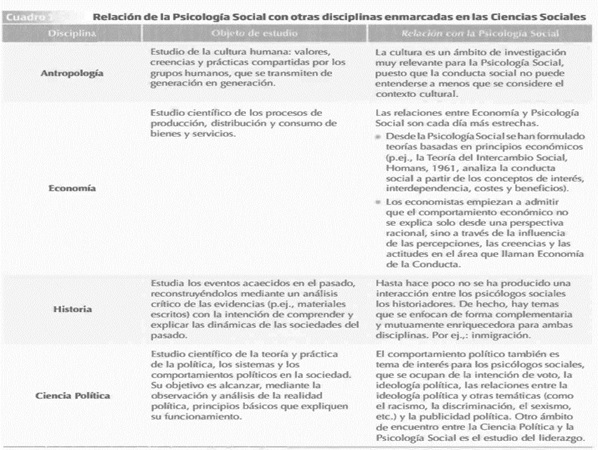
\includegraphics[keepaspectratio]{static/images/image1.png}}
\caption{Relación de la Psicología Social con otras disciplinas}
\end{figure}

\section*{2. Principios básicos de la Psicología social}\label{tema2}
\addcontentsline{toc}{section}{2. Principios básicos de la Psicología social}

La psicología social sigue unos principios básicos que influyen en la investigación de los psicólogos sociales, es decir, la forma en la que estos se acercan a los temas de estudio, la manera en que formulan las hipótesis de sus investigaciones y el modo en que evalúan el comportamiento social.

\subsection*{2.1 Construimos nuestra realidad social}\label{subtema2_1}
\addcontentsline{toc}{subsection}{2.1 Construimos nuestra realidad social}

Las personas nos esforzamos por darle sentido a la realidad de forma que nos resulte ordenada, predecible y controlable. La forma en la que reaccionamos a esta realidad no depende sólo de hechos objetivos, sino de la interpretación que hacemos sobre ellos. Ello explica por qué las personas reaccionamos diferente ante los mismos acontecimientos: no están en presencia del mismo fenómeno debido a que lo han interpretado de manera diferente.

A menudo, las personas ven lo que quieren ver. Creemos que hay una realidad objetiva ahí fuera, pero la vemos a través de nuestros intereses, motivaciones, actitudes, valores y creencias. Por tanto, la realidad social es subjetiva y construida por cada individuo.

\begin{center}\rule{0.5\linewidth}{0.5pt}\end{center}

\paragraph*{Los movimientos de protesta (Kahan, 2012)}\label{los-movimientos-de-protesta-kahan-2012}
\addcontentsline{toc}{paragraph}{Los movimientos de protesta (Kahan, 2012)}

Este experimento explora cómo los valores a los que cada persona se adhiere influyen en su percepción de los hechos, en situaciones que tienen consecuencias penales.

Se evaluaron los valores más importantes para los participantes, diferenciando entre \textbf{tradicionales} y \textbf{progresistas}. Luego, se mostraron vídeos de una manifestación en la que los manifestantes se enfrentaban a la policía que intentaba dispersarlos.

\textbf{\emph{Condiciones Experimentales}}

\begin{itemize}
\tightlist
\item
  \textbf{Condición clínica de abortos}: A la mitad de los participantes se les informó que la manifestación ocurría frente a una clínica de abortos y que el objetivo era reclamar la legalización del aborto (valores más tradicionales).
\item
  \textbf{Condición centro de reclutamiento militar}: A la otra mitad se les informó que la manifestación ocurría frente a un centro de reclutamiento militar, con el objetivo de protestar contra la prohibición de reclutar soldados abiertamente homosexuales (valores más progresistas).
\end{itemize}

\textbf{\emph{Objetivo del Experimento}}

El objetivo era examinar si los participantes con valores opuestos tendrían percepciones diferentes cuando se les asignaban la misma condición experimental y se les preguntaba sobre el comportamiento de la policía.

\textbf{\emph{Resultados}}

A pesar de que todos vieron el mismo vídeo, la interpretación de lo que observaron ---ya fuera expresiones de disidencia con la intención de persuadir o intimidación física calculada--- dependía de la congruencia entre las posiciones de los manifestantes y los valores culturales de los propios participantes.

\begin{center}\rule{0.5\linewidth}{0.5pt}\end{center}

Las personas tienden a explicar las conductas de los demás recurriendo a características personales, subestimando la influencia de la situación. Sin embargo, la forma en la que se define la situación y las normas sociales imperantes en ella influyen en el comportamiento de las personas.

Las definiciones de la situación y de las normas e ideologías proporcionan un sentido compartido de lo que está bien y lo que está mal (conservadurismo político y liberalismo, el sexismo y racismo\ldots), afectan las percepciones de las personas sobre lo que es y lo que debería ser. Por lo que las creencias, valores y conductas deben entenderse en su contexto social y cultural.

\begin{center}\rule{0.5\linewidth}{0.5pt}\end{center}

\paragraph*{El Dilema del Prisionero: Juego de Wall Street vs Juego de la Comunidad}\label{el-dilema-del-prisionero-juego-de-wall-street-vs-juego-de-la-comunidad}
\addcontentsline{toc}{paragraph}{El Dilema del Prisionero: Juego de Wall Street vs Juego de la Comunidad}

Otro experimento investigó cómo la etiqueta de un juego influía en las decisiones de cooperación. A los participantes se les dijo que jugarían un juego de negociación, pero a algunos se les dijo que era el ``Juego de Wall Street'' y a otros el ``Juego de la Comunidad''.

El resultado fue que el nombre del juego influyó significativamente en las decisiones de los participantes. En el Juego de la Comunidad, tanto los participantes cooperativos como los competitivos cooperaron, mientras que en el Juego de Wall Street sólo el 33\% cooperaron, independientemente de su personalidad.

Por otro lado, el hecho de que los participantes que cooperaron recibiesen cooperación en la primera ronda, generalmente influía a que cooperasen en las siguientes rodas, mientras que los que habían competido o se enfrentaban a competencia tendieron a competir desde entonces.

\begin{center}\rule{0.5\linewidth}{0.5pt}\end{center}

\subsubsection*{El Dilema del Prisionero}\label{cuadro2_1}
\addcontentsline{toc}{subsubsection}{El Dilema del Prisionero}

\begin{center}\rule{0.5\linewidth}{0.5pt}\end{center}

El Dilema del Prisionero es un problema fundamental de la teoría de juegos que comenzó en el ámbito de las matemáticas. Este dilema describe una situación en la que dos personas pueden elegir no cooperar, a pesar de que si lo hicieran, obtendrían un resultado más beneficioso para ambas partes.

En el escenario clásico, la policía arresta a dos sospechosos de un crimen y les ofrece el mismo trato por separado:

\begin{itemize}
\tightlist
\item
  Si uno confiesa y su cómplice no lo hace, el cómplice será condenado a cinco años de prisión mientras que el delator será liberado.
\item
  Si ambos confiesan, cada uno recibe una condena de cuatro años.
\item
  Si ninguno confiesa, ambos pasarán solo un año en prisión por falta de pruebas.
\end{itemize}

Desde la perspectiva de uno de los sospechosos, la mejor opción individual es confesar, ya que le beneficia haga lo que haga la otra persona. Sin embargo, si ambos cooperan y no confiesan, serán condenados solo a un año cada uno, lo que sería el mejor resultado conjunto.

Este juego se puede hacer en una sola ronda, pero presenta mayor interés cuando hay varias rondas, ya que les permite a los jugadores aprender progresivamente y ajustar su conducta en función de las acciones del otro.

\subsection*{2.2 Los motivos sociales}\label{subtema2_2}
\addcontentsline{toc}{subsection}{2.2 Los motivos sociales}

Los seres humanos han desarrollado un repertorio de mecanismos psicológicos que permiten la vida social. Estos mecanismos incluyen diversas motivaciones sociales que preparan a las personas para implicarse en acciones colectivas y facilitar la vida en grupo.

\paragraph*{Motivos sociales según Susan Fiske}\label{motivos-sociales-seguxfan-susan-fiske}
\addcontentsline{toc}{paragraph}{Motivos sociales según Susan Fiske}

Susan Fiske argumenta que aquellos que se vinculan adecuadamente con el grupo aumentan enormemente sus posibilidades de supervivencia social. El fracaso en cumplir estos motivos puede tener graves consecuencias para la persona, como exclusión, depresión, ansiedad, e incluso una mayor propensión al suicidio.

\paragraph*{Los principales motivos sociales son:}\label{los-principales-motivos-sociales-son}
\addcontentsline{toc}{paragraph}{Los principales motivos sociales son:}

\begin{itemize}
\tightlist
\item
  \textbf{Pertenencia}: Deseo de establecer y mantener relaciones sociales estrechas con otros. Este motivo reduce las motivaciones individualistas y promueve la conformidad con los roles y normas del grupo. La lealtad hacia el grupo puede intensificar cuando el grupo se ve amenazado.
\item
  \textbf{Comprensión colectiva o compartida}: Necesidad de una visión común del mundo, compartida con otros miembros del grupo.
\item
  \textbf{Control}: Necesidad de poder influir en el entorno social y los resultados de las interacciones sociales.
\item
  \textbf{Perfeccionamiento de sí mismo}: El deseo de mantener una autoestima positiva, ser percibido como bueno y competente dentro del grupo.
\item
  \textbf{Confianza}: La necesidad de confiar en que los demás actuarán de manera predecible y benevolente en el entorno social.
\end{itemize}

Estos motivos sociales son adaptativos y están diseñados para aumentar las posibilidades de supervivencia en un grupo social.

\begin{longtable}[]{@{}
  >{\raggedright\arraybackslash}p{(\linewidth - 0\tabcolsep) * \real{1.0000}}@{}}
\toprule\noalign{}
\endhead
\bottomrule\noalign{}
\endlastfoot
Ejemplo: Apego al grupo en tiempos de crisis \\
Los experimentos han demostrado que el apego al grupo se desarrolla rápidamente, especialmente cuando el grupo se ve amenazado. Un ejemplo de esto se observó en familias de veteranos de la Segunda Guerra Mundial, donde las lealtades grupales se intensificaron en tiempos de crisis. \\
\end{longtable}

\subsubsection*{1 Pertenencia}\label{subtema2_2_1}
\addcontentsline{toc}{subsubsection}{1 Pertenencia}

Subyace a los otros cuatro motivos. Es el deseo imperioso, altamente adaptativo, de adquirir y mantener relaciones sociales estrechas con otros grupos, ser parte de un grupo y llevarse bien con el grupo. Este motivo sirve para reducir las motivaciones individualistas.

El deseo de pertenecer también produce conformidad con los roles y normas dentro del grupo. Las lealtades hacia el grupo pueden dar lugar a hostilidad hacia aquellos que lo amenazan.

\begin{quote}
Cuando el grupo se ve amenazado, la motivación de pertenencia se intensifica.
\end{quote}

\textbf{Experimentos:} El apego al grupo se desarrolla rápidamente, como en el caso de familias de veteranos de la Segunda Guerra Mundial.

\subsubsection*{2 Comprensión colectiva o compartida}\label{subtema2_2_2}
\addcontentsline{toc}{subsubsection}{2 Comprensión colectiva o compartida}

Se relaciona estrechamente con la pertenencia. Es la necesidad de entender lo que creen los otros miembros del grupo o de llegar a un acuerdo compartido en la forma de ver el mundo. Esto permite a las personas predecir lo que sucederá en el futuro y entender lo que sucede en el presente.

Al pertenecer, se confía más en la conceptualización del mundo social dentro del grupo que en la de aquellos individuos que no pertenecen a él. Formar parte del grupo depende de percibir el mundo de la misma manera que los demás; de lo contrario, no se podría pertenecer, y se fomenta que las formas de ver la realidad de los que no pertenecen sean consideradas sesgadas o prejuiciosas.

Las investigaciones empíricas promueven la existencia universal de un motivo de comprensión compartida, pero hay líneas de investigación para explicar sus diferencias:

\begin{itemize}
\tightlist
\item
  \textbf{Colectivistas:} Enfatizan el acuerdo armonioso y unánime.
\item
  \textbf{Individualistas:} Toleran interpretaciones individuales, incluso si van en contra del consenso social.
\end{itemize}

La falta de comprensión colectiva se refleja en la falta de información y poder de los miembros que no están adecuadamente integrados en el grupo. En las primeras etapas de pertenencia, se busca información sobre las normas del grupo y el papel que desempeñan los individuos dentro de él. Si no se logra una comprensión compartida, pueden mostrar conductas desviadas que los ponen en riesgo de devaluación, un componente central de la exclusión social.

\subsubsection*{3 Control}\label{subtema2_2_3}
\addcontentsline{toc}{subsubsection}{3 Control}

El motivo de control se refiere a la necesidad de tener influencia sobre el entorno y los resultados sociales de nuestros comportamientos. Las personas prestan más atención a aquellos que tienen control sobre ellas, lo que refuerza aún más este motivo. Además, se implican en procesos cognitivos más complejos para entender a las personas de las que dependen para sus resultados sociales.

El motivo de control fomenta la exclusión por dos vías principales:

\begin{itemize}
\tightlist
\item
  \textbf{Vigilancia} de aquellos grupos externos que pueden amenazar la autonomía dentro del grupo.
\item
  \textbf{Ignorancia} hacia aquellos que no tienen influencia en sus resultados.
\end{itemize}

\subsubsection*{4 Perfeccionamiento de sí mismo}\label{subtema2_2_4}
\addcontentsline{toc}{subsubsection}{4 Perfeccionamiento de sí mismo}

El perfeccionamiento de sí mismo se refiere a la necesidad de sentirse bien consigo mismo, mantener una autoestima razonablemente alta y verse a uno mismo como bueno, competente y decente.

En situaciones donde hay que elegir entre distorsionar la realidad para sentirse bien o percibir el mundo con precisión, la mayoría de las personas elige la primera opción. Para mantener una imagen positiva de sí mismos, están dispuestas a hacer cosas sorprendentes o paradójicas, como preferir a personas y situaciones que les han causado sufrimiento en lugar de aquellas que les agradan, si eso contribuye a su perfeccionamiento personal (por ejemplo, tolerar novatadas para ser aceptados).

Los seres humanos emplean un \textbf{sociometro}, que es un mecanismo que indica su posición dentro del grupo y les ayuda a vigilar su autoestima.

El motivo de perfeccionamiento de sí mismo es a menudo difícil de satisfacer, incluso para aquellos que son aceptados. Cuando las personas enfrentan amenazas en áreas relevantes para su autoestima, tienden a socavar sus relaciones interpersonales, lo que puede provocar emociones negativas como ira, tristeza o vergüenza, y una tendencia a centrarse en sí mismos, desviando la atención de los objetivos grupales.

\subsubsection*{5 Confianza}\label{subtema2_2_5}
\addcontentsline{toc}{subsubsection}{5 Confianza}

La confianza satisface la necesidad social de percibir el mundo como un lugar benevolente. Formar vínculos estrechos implica tener fe y confianza dentro del grupo. Las personas que confían ven la realidad social de forma más benévola y, como resultado, son más empáticas.

Confiar conlleva la contrapartida de excluir a otros, ya que las personas comparan a los miembros del grupo que son fiables con aquellos en quienes supuestamente no se puede confiar.

\begin{itemize}
\item
  \textbf{Individualistas:} La confianza se da por descontado. Se considera que todos son confiables y benignos hasta que se demuestre lo contrario. Esto se puede inferir incluso a partir de rasgos faciales en exposiciones muy breves, de menos de 100 milisegundos.
\item
  \textbf{Colectivistas:} El círculo de confianza suele ser más estrecho y limitado a familiares cercanos y vínculos personales y profesionales consolidados. Tener confianza en los demás permite una mayor satisfacción con la realidad social, menos resentimiento, más éxito social y menos soledad.
\end{itemize}

La falta de confianza puede dañar la capacidad de formar relaciones constructivas. Por ejemplo, las personas traicionadas pueden volverse ultrasensibles al comportamiento de los demás, siendo más propensas a mentir, engañar y robar. También es menos probable que den una segunda oportunidad o que respeten los derechos de los demás.

\textbf{Marco de BUCKET:} Pertenencia, comprensión, control, estima y confianza.

Investigaciones recientes han tratado de analizar si los motivos sociales son válidos en distintas culturas. Los resultados mostraron que en países asiáticos (colectivistas), el motivo de pertenencia fue el más alto. Por otro lado, las amenazas sociales percibidas, el cambio cultural o el avance tecnológico correlacionan positivamente con todos los motivos sociales clave, aunque el vínculo más fuerte es con el motivo de control.

\begin{center}\rule{0.5\linewidth}{0.5pt}\end{center}

\paragraph*{Resumen de los motivos sociales centrales}\label{subtema2_2_6}
\addcontentsline{toc}{paragraph}{Resumen de los motivos sociales centrales}

En resumen, los cinco motivos sociales centrales se orientan al bienestar personal, a través de la aceptación y el éxito dentro del grupo:

\begin{itemize}
\item
  \textbf{Pertenencia:} La primera meta es sentir que uno ha logrado un lugar seguro dentro del grupo, estableciendo lazos sociales fuertes con los demás miembros.
\item
  \textbf{Comprensión colectiva:} Las personas dentro del grupo comparten una visión del mundo social, que es constantemente reforzada por otros miembros.
\item
  \textbf{Control:} Creen que su conducta social tiene una influencia directa en los resultados que consiguen.
\item
  \textbf{Perfeccionamiento de sí mismo:} Al pertenecer al grupo, los miembros se sienten bien consigo mismos y ven oportunidades para desarrollarse.
\item
  \textbf{Confianza:} Se fomenta un ambiente de confianza entre los miembros del grupo.
\end{itemize}

Por el contrario, la situación es desfavorable para los excluidos de los grupos, ya que se enfrentan a la insatisfacción de sus motivos sociales y sus expectativas sobre el mundo social pueden estar dañadas, a veces irreparablemente.

\begin{center}\rule{0.5\linewidth}{0.5pt}\end{center}

\subsection*{2.3 La interconexión de los procesos psicosociales}\label{subtema2_3}
\addcontentsline{toc}{subsection}{2.3 La interconexión de los procesos psicosociales}

La Psicología Social se centra en estudiar los pensamientos, sentimientos y comportamientos de las personas en relación con su ambiente social, lo que da lugar a procesos que se pueden analizar en diferentes niveles de explicación. Esto se refiere a los conceptos, mecanismos y lenguajes usados para explicar un fenómeno.

\textbf{\emph{Niveles de procesos psicosociales}}

\begin{enumerate}
\def\labelenumi{\arabic{enumi}.}
\tightlist
\item
  \textbf{Procesos Intrapersonales}:
  Tienen lugar en el interior de una persona en relación con el ambiente social (en presencia de otras personas, reales o no). Incluyen procesos intrapsíquicos, emocionales o motivacionales. Incluso en la intimidad, influyen los demás a través de normas sociales o expectativas externas.

  \begin{itemize}
  \tightlist
  \item
    \textbf{Autoestima personal}: Sentimiento sobre la propia valía.
  \item
    \textbf{Proceso atributivo intrapersonal}: Asignación de éxitos personales a uno mismo y de fracasos a factores externos o a otras personas.
  \end{itemize}
\item
  \textbf{Procesos Interpersonales (y Situacionales)}:
  Se refieren a la interacción entre dos personas, siempre que estén relacionándose en su condición individual, no como miembros de un grupo. Aquí no se consideran las posiciones fuera de la situación.

  \begin{itemize}
  \tightlist
  \item
    Ejemplo: Relaciones íntimas como el amor o la amistad.
  \end{itemize}
\item
  \textbf{Procesos Grupales (Posicionales)}:
  Involucran la interacción entre individuos en función de su pertenencia a grupos sociales. Aquí se toma en cuenta el estatus dentro del grupo y la identidad social fuera de la situación específica.

  \begin{itemize}
  \tightlist
  \item
    \textbf{Liderazgo según la Teoría de la Identidad Social (TIS)}: Reconoce el papel del líder y de los seguidores como miembros de un grupo. El liderazgo se entiende como una relación entre líderes y seguidores en un contexto grupal.
  \end{itemize}
\item
  \textbf{Procesos Macrosociales (Ideológicos)}:
  Se analizan interacciones individuales o grupales, pero se considera el papel de las normas sociales y las relaciones entre grupos. Un ejemplo sería la influencia cultural en conductas agresivas.
\end{enumerate}

\subsubsection*{2.3.1 Críticas al reduccionismo en Psicología Social}\label{subtema2_3_1}
\addcontentsline{toc}{subsubsection}{2.3.1 Críticas al reduccionismo en Psicología Social}

Las críticas al reduccionismo hacen referencia a que la explicación de un fenómeno se hace usando conceptos de un nivel de análisis inferior, lo que conlleva una pérdida de poder explicativo. Por ejemplo, explicar un fenómeno grupal usando procesos interpersonales puede dejar sin respuesta preguntas relativas a un nivel superior.

Ejemplo del concejal romano y el saludo fascista: Si un concejal romano realiza un saludo fascista en un funeral y es criticado, explicar su acción como una contracción muscular reduce la explicación a niveles biológicos. No se considera el simbolismo histórico y el significado de pertenecer a grupos de ultraderecha.

Por lo tanto, explicaciones del comportamiento social que solo aluden a procesos cognitivos o neurociencia cognitiva social pueden ser criticadas por este motivo.

\paragraph*{Tipos de procesos psicosociales en función del nivel de explicación del comportamiento social}\label{tipos-de-procesos-psicosociales-en-funciuxf3n-del-nivel-de-explicaciuxf3n-del-comportamiento-social}
\addcontentsline{toc}{paragraph}{Tipos de procesos psicosociales en función del nivel de explicación del comportamiento social}

\begin{figure}
\centering
\pandocbounded{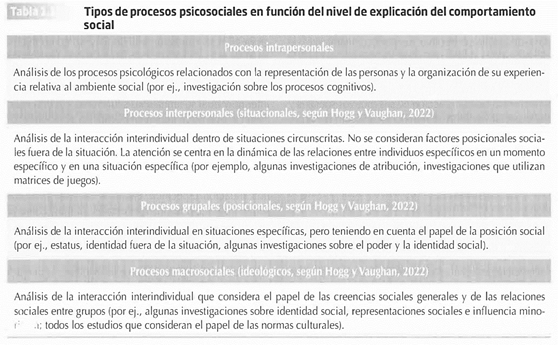
\includegraphics[keepaspectratio]{static/images/image2.png}}
\caption{Tipos de procesos psicosociales}
\end{figure}

\subsubsection*{2.3.2 La conexión entre los procesos psicosociales}\label{subtema2_3_2}
\addcontentsline{toc}{subsubsection}{2.3.2 La conexión entre los procesos psicosociales}

Los procesos psicosociales de diferentes niveles forman una red de relaciones complejas, donde los procesos grupales pueden afectar a los interpersonales. Un ejemplo es la transmisión cultural individualista/colectivista, que ilustra cómo se transmiten las orientaciones culturales a los inmigrantes de segunda generación y la relación entre estas formas de transmisión y las diferencias cognitivas entre inmigrantes y grupos nativos.

Las personas de los países WEIRD (Occidentales, Educados, Industrializados, Ricos y Democráticos) muestran un procesamiento cognitivo diferente: mayor individualismo, que se traduce en una cognición más analítica y menos holística. Sin embargo, los mecanismos para mantener esta diferencia cultural entre inmigrantes de segunda generación no están claros.

Los investigadores han diferenciado entre varios mecanismos de transmisión cultural:

\begin{itemize}
\tightlist
\item
  \textbf{Transmisión cultural vertical:} Aprender de los padres.
\item
  \textbf{Transmisión cultural oblicua:} Aprender de otros mayores que no son los padres, como maestros u otros familiares.
\item
  \textbf{Transmisión cultural horizontal:} Aprender de los compañeros.Subprocesos:

  \begin{itemize}
  \tightlist
  \item
    \textbf{Conformidad:} Adoptar los comportamientos mayoritarios.
  \item
    \textbf{Sesgo de prestigio:} Imitar a personas famosas.
  \item
    \textbf{Transmisión de uno a muchos:} A través de los medios de comunicación.
  \end{itemize}
\end{itemize}

Hay evidencia de que la transmisión cultural horizontal puede ser tan influyente como la vertical o incluso más.

\paragraph*{Estudio de Mesoudi et al.~(2016)}\label{estudio-de-mesoudi-et-al.-2016}
\addcontentsline{toc}{paragraph}{Estudio de Mesoudi et al.~(2016)}

Mesoudi et al.~realizaron un estudio sobre los mecanismos de transmisión cultural individualista que ejemplifica cómo se pueden estudiar simultáneamente procesos intrapersonales (estilos cognitivos de atribución) con procesos macrosociales (orientación cultural).

El estudio se centró en inmigrantes bangladesíes, cuyos resultados mostraron que el individualismo y la \textbf{atribución disposicional} (tendencia a explicar los comportamientos de otros a partir de sus características personales) típicos de las sociedades occidentales se deben a la transmisión cultural horizontal, que se transmite más rápidamente, mientras que los padres u otros miembros familiares ejercen poca o ninguna influencia.

En cambio, el colectivismo, la cercanía social y la \textbf{atribución situacional} (tendencia a explicar los comportamientos de otros a partir de sus circunstancias ambientales) fueron impulsados por una combinación de transmisión vertical, oblicua y horizontal.

\subsubsection*{2.3.3 El efecto de discontinuidad individuo-grupo}\label{subtema2_3_3}
\addcontentsline{toc}{subsubsection}{2.3.3 El efecto de discontinuidad individuo-grupo}

El efecto de discontinuidad individuo-grupo se refiere a la tendencia de que las relaciones entre grupos sean más competitivas que las relaciones entre individuos. En el dilema del prisionero, la explicación para seguir una estrategia competitiva en la relación intergrupal puede agruparse en varios conjuntos: codicia y miedo.

\begin{itemize}
\item
  \textbf{Codicia:} Se espera que el contrincante coopere, haciéndolo más vulnerable.
\item
  \textbf{Miedo:} Se espera que el contrincante compita y, por lo tanto, se convierta en una amenaza.
\end{itemize}

Por lo tanto, la codicia y el miedo pueden ser mayores en las relaciones entre grupos que en las interpersonales.

Otra explicación es que el grupo promueve el \textbf{egoísmo}, brindando apoyo social a estas conductas, mientras que este apoyo no está disponible para los individuos que actúan de forma aislada.

Además, el \textbf{anonimato} proporcionado por los grupos, que no existe en las relaciones interpersonales, también contribuye a este fenómeno.

Finalmente, hay una \emph{desconfianza} basada en \emph{esquemas.} Al interactuar con otros grupos, se activan esquemas basados en el aprendizaje previo que nos llevan a \emph{interacciones competitivas}, actuando de acuerdo con tales expectativas.

\subsection*{2.4 Comportamiento social y cognición social}\label{subtema2_4}
\addcontentsline{toc}{subsection}{2.4 Comportamiento social y cognición social}

Hoy en día, el comportamiento y la cognición social se consideran fenómenos estrechamente relacionados. No es posible estudiar uno sin el otro; para comprender cómo las personas se comportan en situaciones sociales, se deben considerar sus pensamientos, memoria, intenciones, emociones, actitudes y creencias. A su vez, las consecuencias de estas acciones afectan nuestras emociones y pensamientos.

\paragraph*{Evolución de la cognición social}\label{evoluciuxf3n-de-la-cogniciuxf3n-social}
\addcontentsline{toc}{paragraph}{Evolución de la cognición social}

En la primera etapa de los años 80, las personas eran vistas como ``ahorradores'' con escasa capacidad de procesamiento, propensas a tomar atajos (heurísticos). Se abandona la idea del ser humano como completamente racional, y la investigación se centra en dos procesos:

\begin{itemize}
\item
  \textbf{Saliencia:} La información que destaca sobre otras.
\item
  \textbf{Uso de categorías sociales:} Los observadores clasifican a las personas según categorías como raza o género, ignorando su individualidad (tacaño cognitivo).
\end{itemize}

En los años 90, se reconoció que la cognición social es útil para la interacción social. Ideas clave incluyen:

\begin{enumerate}
\def\labelenumi{\arabic{enumi}.}
\tightlist
\item
  Al percibir a otros, usamos estrategias suficientemente buenas para alcanzar nuestras metas cotidianas.
\item
  Construimos significados que van más allá de la información dada, a través de conceptos como rasgos, estereotipos o historias (estrategas motivados).
\end{enumerate}

\paragraph*{Modelo de procesamiento dual (Fiske y Neuberg, 1999)}\label{modelo-de-procesamiento-dual-fiske-y-neuberg-1999}
\addcontentsline{toc}{paragraph}{Modelo de procesamiento dual (Fiske y Neuberg, 1999)}

Este modelo aborda cuándo las personas utilizan estrategias rápidas y cuándo se involucran en procesos más detallados. Los perceptores forman impresiones inicialmente usando atajos, categorizando a las personas según \emph{características sobresalientes} (género, edad) y priorizando esas impresiones.

Si la impresión es suficiente para su objetivo cotidiano (interactuar con un camarero), el proceso se detiene.

Si el ajuste no es bueno (por ejemplo, el género del camarero es ambiguo) o la motivación es alta (el camarero es amigo de un amigo), se prestará más atención, lo que puede transformar las impresiones basadas en estereotipos en impresiones más individualizadas.

\paragraph*{Etapa presente}\label{etapa-presente}
\addcontentsline{toc}{paragraph}{Etapa presente}

En la actualidad, donde la desigualdad es objeto de interés, la cognición social ve a las personas como facilitadores de la desigualdad. El concepto de ``envidia hacia arriba, desprecio hacia abajo'' se refiere a cómo el estatus nos divide (Fiske, 2010). Los procesos cognitivos sociales, como sesgos y atajos, no causan desigualdad, pero permiten que exista a nivel interpersonal.

\begin{itemize}
\item
  Las personas de alto estatus intentan proyectar calidad y tienden a hablar con personas de menor estatus, minimizando su propia competencia.
\item
  Si se preocupan por parecer justos e igualitarios, pueden patrocinar a las personas menos privilegiadas.
\end{itemize}

Los trabajos de Taylor sobre la salud y de Fiske en el laboratorio se centran en las \emph{familias} como sustentadoras de la \emph{desigualdad.} Aunque la familia se considera un entorno cálido y protector, no siempre es así.

\begin{longtable}[]{@{}
  >{\raggedright\arraybackslash}p{(\linewidth - 0\tabcolsep) * \real{1.0000}}@{}}
\toprule\noalign{}
\endhead
\bottomrule\noalign{}
\endlastfoot
Resumen \\
* \textbf{Tacaño cognitivo (80s):} Uso de atajos mentales para conservar los recursos cognitivos. \\
* \textbf{Estratega motivado (90s):} Destaca cómo las influencias motivacionales y situacionales pueden influir en las estrategias cognitivas que se emplean para procesar la información social. \\
* \textbf{Actor activo (2000s):} El papel del entorno social en la provocación de objetivos y la formación de respuestas, donde las acciones basadas en objetivos son activadas situacionalmente. \\
* \textbf{Facilitador de la desigualdad (2010s):} Las personas apoyamos estereotipos y juicios hacia los demás que establecen quién es bueno y quién es malo. \\
\end{longtable}

\subsection*{2.5 El papel de la emoción en la Psicología Social}\label{subtema2_5}
\addcontentsline{toc}{subsection}{2.5 El papel de la emoción en la Psicología Social}

Las emociones son sentimientos complejos que nos proporcionan información valiosa y nos ayudan a actuar para sobrevivir. Tradicionalmente, la cognición y la emoción se han trabajado de forma paralela en la Psicología Social, a menudo con más visibilidad dada a la cognición.

Es en la etapa de los \emph{actores activados} cuando se comienza a estudiar las respuestas afectivas a través de patrones neuronales, actividad muscular y otros indicadores. Estos estudios han mostrado que el afecto y la cognición, en conjunto, predicen el comportamiento de manera más eficaz que al emplear únicamente la cognición.

\subsection*{2.6 Importancia de las relaciones sociales para el bienestar de las persona}\label{subtema2_6}
\addcontentsline{toc}{subsection}{2.6 Importancia de las relaciones sociales para el bienestar de las persona}

La importancia de las relaciones sociales para el bienestar de las personas es un tema que se basaba en el sentido común y la experiencia personal, pero que ha comenzado a investigarse científicamente en las últimas décadas.

La reducción de las familias extensas en el mundo occidental y la decisión de muchas personas adultas de pasar parte de su vida adulta solas, sin que esto signifique un menoscabo de su bienestar, han motivado estas investigaciones.

\paragraph*{Evidencias}\label{evidencias}
\addcontentsline{toc}{paragraph}{Evidencias}

\begin{itemize}
\item
  \textbf{Biológica:} Cuando hay un sentido de identidad social compartida dentro de un grupo, se amortigua el estrés neuroendocrino.
\item
  Pertenecer a muchos \textbf{grupos} (familia, trabajo, universidad) nos hace más saludables y resilientes.
\item
  Un estudio en atención primaria mostró que el \textbf{aislamiento} tiene efectos negativos para la salud.
\item
  Pertenecer a múltiples grupos sociales se asocia con un mayor \textbf{bienestar} psicológico y una mayor longevidad que pertenecer a pocos grupos sociales.
\end{itemize}

La \textbf{Pertenencia Grupal Múltiple} (MGM, por sus siglas en inglés, Multiple Group Membership) protege a las personas antes de que sucedan cambios importantes en la vida personal. La revisión de la literatura identifica efectos sobre el bienestar en relación con el estrés, la depresión, las adicciones, la conducta alimentaria y problemas crónicos de salud mental o física.

Existen evidencias sólidas de que el contacto social y la pertenencia a grupos tienen una fuerte influencia sobre la salud y la longevidad, mientras que la falta de contacto y el aislamiento constituyen factores de riesgo para una muerte prematura.

\subsection*{2.7 La importancia de la diversidad social}\label{subtema2_7}
\addcontentsline{toc}{subsection}{2.7 La importancia de la diversidad social}

La diversidad de grupos sociales en función de la edad, el género, las creencias religiosas, la etnia, la orientación sexual, la diversidad funcional, la clase social o la cultura, entre otras variables, se ha situado en el centro de atención. De esta forma, hay un análisis más cuidadoso de cómo cambia el comportamiento en función de qué categorías sociales se utilizan para definir el yo en un momento dado.

\begin{center}\rule{0.5\linewidth}{0.5pt}\end{center}

\subsubsection*{Apreciación Corporal: Cultura + Variables Situacionales}\label{apreciaciuxf3n-corporal-cultura-variables-situacionales}
\addcontentsline{toc}{subsubsection}{Apreciación Corporal: Cultura + Variables Situacionales}

\textbf{Estudio transcultural (Swami, 2010) sobre los ideales de peso corporal femenino y la insatisfacción corporal de las mujeres:}
- En las regiones de bajo nivel socioeconómico se mostró preferencia por los cuerpos más pesados.
- La edad, el IMC y la exposición a los medios occidentales pronosticaron los ideales de peso corporal.
- El IMC y la exposición a los medios occidentales pronosticaron la insatisfacción corporal entre mujeres.
- La insatisfacción corporal y el deseo de delgadez son comunes en entornos de alto nivel socioeconómico en todas las regiones del mundo.

\textbf{Estudio: práctica de usar hijab y discrepancia entre peso real e ideal:}
- Las mujeres que usaban hijab tenían menor discrepancia, menor insatisfacción corporal, menor impulso para adelgazar, pero más discriminación.

\textbf{Estudio: poblaciones rurales-urbanas en Malasia:}
- Los participantes rurales tenían una apreciación corporal significativamente mejor que los participantes urbanos. No hay diferencia entre hombres y mujeres.
- En el ámbito urbano los hombres tenían una apreciación corporal mejor que las mujeres.
- La apreciación corporal se asoció con la satisfacción con la vida tanto en entornos rurales como urbanos.

\textbf{Imagen corporal positiva y contacto con la naturaleza:}
- Mujeres que salieron a dar un paseo por el bosque durante 40 minutos en Polonia anotaron su apreciación corporal antes y después del paseo. Fue mejor después del paseo.
- Incluso una exposición breve en la naturaleza produce un estado de apreciación elevado.

\begin{center}\rule{0.5\linewidth}{0.5pt}\end{center}

\section*{3. Cómo responden los psicólogos sociales a las preguntas que se plantean: la investigación en psicología social}\label{tema3}
\addcontentsline{toc}{section}{3. Cómo responden los psicólogos sociales a las preguntas que se plantean: la investigación en psicología social}

Para que un conocimiento sea científico, se requiere que se haya llegado a él a través del método científico. Los Psicólogos Sociales no se contentan con saber qué hacen las personas, sino que quieren saber también por qué lo hacen. Para ello, derivan hipótesis de las teorías.

\subsection*{3.1. Teorías científicas: formulación y puesta a prueba de hipótesis}\label{subtema3_1}
\addcontentsline{toc}{subsection}{3.1. Teorías científicas: formulación y puesta a prueba de hipótesis}

Las teorías científicas son un conjunto de constructos, de ideas abstractas o conceptos que están relacionados entre sí siguiendo una lógica. Además, deben ser contrastables y, para ello, deben definir sus constructos teóricos operativamente. Si no pueden definirse, la teoría va más allá del ámbito de la ciencia.

Un constructo puede tener una o varias dimensiones. Por ejemplo, el constructo \textbf{agresión} puede incluir tanto agresión física o verbal, directa o indirecta, colérica o fría\ldots{} De esta forma, la teoría integra los constructos y explica por qué es esperable que algo suceda de una forma y no en otra.

Los constructos son abstractos e inobservables (no es visible la agresión directamente, sino por medio de conductas agresivas). Por lo que los psicólogos sociales tienen que formular definiciones operativas de los constructos.

A partir de las teorías, los investigadores formulan hipótesis, que son soluciones tentativas a un problema, que deben ser contrastables, es decir, son predicciones formalmente establecidas sobre lo que puede causar que algo ocurra.

\subsection*{3.2. Métodos de investigación en psicología social}\label{subtema3_2}
\addcontentsline{toc}{subsection}{3.2. Métodos de investigación en psicología social}

Los métodos se pueden clasificar en dos grupos: experimentales y no experimentales. La elección dependerá de múltiples factores: de la naturaleza de la hipótesis, de la disponibilidad de recursos (tiempo, financiación, participantes\ldots) y de las limitaciones éticas del método.

La \textbf{experimentación sistemática} es el método preferido por los psicólogos sociales y científicos en general, pero muchas veces resulta imposible de realizar. Por ejemplo, está limitada en cuanto a que las características de las personas no son susceptibles de experimentación (no se puede manipular el sexo biológico y ver qué efectos surgen) o por la existencia de cuestionamientos éticos. Implica la intervención en forma de manipulación de una o más variables, y su posterior medición del efecto de dicha manipulación sobre una o más variables que son las que interesan al investigador.

Cuando no es posible realizar un experimento o no es ético, se deberá recurrir a métodos no experimentales. Estos carecen de una o varias de las características claves del experimento como la manipulación de una variable independiente y la asignación aleatoria de los participantes a las diversas condiciones experimentales, por lo tanto, se limitan al análisis de la relación entre variables que impiden extraer conclusiones causales.

\textbf{Ejemplo:} podríamos tener a dos grupos de personas (unas víctimas de delitos violentos y otras que no lo han sido) para evaluar su autoestima y ver si hay diferencias. Sin embargo, las diferencias se podrían deber al delito o a otras muchas causas no controlables entre ambos grupos, por lo que sólo sería admisible afirmar que existe una relación entre la autoestima y el hecho de haber sido víctima de delitos violentos. Ya que no hay evidencia de que un hecho cause el otro, ser víctima puede bajar la autoestima o la baja autoestima puede hacer que aumente la probabilidad de convertirse en víctima, o puede haber una tercera variable como el desempleo que haya disminuido esta.

El pluralismo metodológico ayuda a reducir la posibilidad de que un resultado encontrado sea efecto de un método particular. La replicación por parte de diferentes grupos de estudio ayuda a evitar el sesgo de confirmación.

\begin{longtable}[]{@{}
  >{\raggedright\arraybackslash}p{(\linewidth - 0\tabcolsep) * \real{1.0000}}@{}}
\toprule\noalign{}
\endhead
\bottomrule\noalign{}
\endlastfoot
\#\#\# El sesgo de confirmación \\
Cuando los investigadores se involucran tan intensamente en sus propias teorías que pierden objetividad en la interpretación de los datos y toman en consideración solo aquellos datos que avalan sus hipótesis, descartando los datos contrarios a ellas. \\
\end{longtable}

\subsection*{3.3. El experimento: generación del conocimiento a través de la intervención sistemática}\label{subtema3_3}
\addcontentsline{toc}{subsection}{3.3. El experimento: generación del conocimiento a través de la intervención sistemática}

El experimento es un procedimiento para probar una hipótesis en el que se hace algo con el objetivo de comprobar qué efecto tiene sobre otra cosa.

La \textbf{variable independiente} es cualquier evento observable que causa que la persona haga algo. Independiente en el sentido de que sus valores son creados o manipulados por el investigador y no se ven afectados por nada más de lo que suceda en el experimento, ni por el propio participante. Es una variable porque tiene al menos dos niveles, categorías, tipos o grupos (frustración y no frustración).

La conducta es una función tanto de la situación como de las diferencias personales, pero mientras que las variables relativas a la situación se pueden manipular (aumentar el calor de la sala para valorar la relación calor-agresión), las variables relativas a las diferencias individuales como el género, edad, inteligencia\ldots{} se pueden medir y nos dan información sobre cómo se correlaciona, pero no se puede manipular. Esto limita en cuanto a que sólo se pueden sacar conclusiones de causalidad (A es causa o efecto de B) sobre las auténticas variables independientes que fueron manipuladas.

Sólo la experimentación puede establecer la causalidad.

La \textbf{variable dependiente} es cualquier comportamiento observable que produce una persona. Es dependiente en el sentido que sus valores dependen de la variable independiente.

\textbf{Ejemplo:} Estudio del efecto de la cerveza con alcohol vs sin alcohol sobre la agresión.
- VD: Agresión
- VI: Cerveza con alcohol vs sin alcohol

Se podrían usar diferentes medidas de agresión: insultos verbales, agresiones físicas\ldots{} y diferentes formas de operativizar la agresión.

\subsubsection*{3.3.1. Control: manipulación de variables (y asignación aleatoria)}\label{subsubtema3_3_1}
\addcontentsline{toc}{subsubsection}{3.3.1. Control: manipulación de variables (y asignación aleatoria)}

Un experimento tiene dos características esenciales:

\begin{enumerate}
\def\labelenumi{\arabic{enumi}.}
\item
  El investigador tiene control sobre los procedimientos → manipula la VI y mantiene constantes todas las demás variables, tiene que asegurarse de que cualquier diferencia observada en la VD es causada por la VI y no por otros factores. De esta forma, el investigador tiene la responsabilidad de hacer el experimento creíble para los participantes.
\item
  Los participantes son asignados aleatoriamente → donde tengan la misma oportunidad de ser asignados en cada grupo. De esta forma, los participantes de cada grupo se espera que sean similares a los del otro grupo, así tras manipular la variable independiente se espera que las diferencias entre los grupos sean el resultado de la variable independiente y no de diferencias iniciales preexistentes entre los participantes.
\end{enumerate}

\textbf{Tipos de manipulaciones experimentales y verificación de la manipulación}

\begin{enumerate}
\def\labelenumi{\arabic{enumi}.}
\tightlist
\item
  \textbf{Manipulación ambiental}: se modifican características del entorno (iluminación, ruido de fondo, temperatura\ldots).
\end{enumerate}

\textbf{Ejemplo:} Descargas eléctricas y presencia de armas (agresión).

Se expuso a los participantes a descargas eléctricas (entre 1 a 7 descargas). Después, tenían la oportunidad de administrar descargas a quienes les habían electrocutado previamente. En unas condiciones se colocó sobre la mesa un arma, en otras en la mesa había unas raquetas de bádminton o no había nada. \textbf{Resultado}: Los participantes en presencia de armas aplicaron más descargas que los de la raqueta o control (nada) si habían estado en la condición de descarga máxima (7 descargas).

\begin{enumerate}
\def\labelenumi{\arabic{enumi}.}
\setcounter{enumi}{1}
\tightlist
\item
  \textbf{Manipulación mediante estímulo}: modificación del material visual o verbal proporcionado a los participantes.
\end{enumerate}

\textbf{Ejemplo:} Estereotipo mujeres y matemáticas.

Se trató de comprobar el efecto de la amenaza del estereotipo sobre las mujeres para la realización de tareas de matemáticas. Se repartió un ejercicio de cálculo igual para todas las condiciones. Después, apareció el estímulo modificado: se repartió una noticia del periódico (neutra para los varones, y manipulada para las mujeres donde leen que se ha demostrado que las mujeres rinden peor en las tareas de cálculo). Se vuelve a repartir un ejercicio de cálculo igual que en la primera fase.

\begin{enumerate}
\def\labelenumi{\arabic{enumi}.}
\setcounter{enumi}{2}
\tightlist
\item
  \textbf{Manipulación social}: se modifican las características sociales mediante la presencia o ausencia de otras personas y su comportamiento durante el experimento.
\end{enumerate}

\textbf{Ejemplo:} Grado de conformidad.

Se juntaban a participantes con colaboradores del experimentador (el participante pensaba que era otro participante ajeno al experimentador). La tarea consistía en comparar una línea con otras y decir cuál era la que era igual en longitud, siendo la respuesta muy obvia para cualquier persona. \textbf{Resultado}: Los participantes podían resistir la influencia del grupo cuando decían la respuesta errónea solamente cuando había uno o dos cómplices, si había tres o más aumenta dramáticamente el grado de conformidad (cuando se añaden más de tres no hay un aumento significativo respecto a tres).

\begin{enumerate}
\def\labelenumi{\arabic{enumi}.}
\setcounter{enumi}{3}
\tightlist
\item
  \textbf{Manipulación mediante instrucciones}: es la forma más común de manipulación experimental. Se manipulan ligeramente las instrucciones proporcionadas a los diferentes grupos de estudio.
\end{enumerate}

\textbf{Ejemplo:} Inicio del video y persuasión.

A un grupo de adolescentes de sexto curso se les muestra un vídeo informando sobre el uso de las drogas. A un grupo le muestra un vídeo que comienza con ``Padres, ¿tenéis un adolescente en casa?'' y al otro grupo uno con ``¿estás en sexto curso?'' el resto del vídeo era igual.

\textbf{Resultado}: El vídeo dirigido a los padres causó mucha más persuasión.

\begin{enumerate}
\def\labelenumi{\arabic{enumi}.}
\setcounter{enumi}{4}
\tightlist
\item
  \textbf{Manipulación de activación, preparación o primming}: una tarea que produce un estado mental que a su vez afecta la reacción al siguiente estímulo.
\end{enumerate}

\textbf{Ejemplo:} Bolígrafo labios o dientes.

A un grupo de personas se les asigna sostener un bolígrafo con los labios (impide sonreír) y a otros con los dientes (posición similar a la sonrisa) y se les pone unos dibujos que tienen que valorar como divertidos.

\textbf{Resultado}: Las personas calificaron como más divertidas cuando sostenían con los dientes (sonreían).

\textbf{Verificación de manipulación o manipulation check}

Se trata de una prueba para determinar la efectividad de una manipulación en un diseño experimental. Sirven para comprobar que los participantes perciben, comprenden y reaccionan como se espera a la parte de la manipulación experimental de la VI y consiste en una o varias preguntas para evaluar si los participantes notaron la manipulación. Normalmente, se hacen al final del experimento para no llamar la atención de la manipulación y asegurarse el efecto de esta.

Las comprobaciones de manipulación se vuelven especialmente importantes cuando la manipulación de la VI resulta no tener ningún efecto sobre la VD.

\subsubsection*{3.3.2. Experimentos de laboratorio}\label{subsubtema3_3_2}
\addcontentsline{toc}{subsubsection}{3.3.2. Experimentos de laboratorio}

El experimento social se lleva a cabo en un laboratorio ya que permite controlar las variables extrañas. Lo más relevante es que su validez interna (realismo experimental) sea elevada, que las manipulaciones realizadas sean significativas y tengan impacto psicológico para los participantes.

El objetivo no es conocer la conducta de las personas en el laboratorio, sino poner a prueba las hipótesis derivadas de las teorías sobre el comportamiento humano.

\textbf{Inconvenientes:} al ser condiciones artificiales y controladas, los resultados no pueden generalizarse directamente a las condiciones del mundo real.

\subsubsection*{3.3.3. Experimentos de campo}\label{subsubtema3_3_3}
\addcontentsline{toc}{subsubsection}{3.3.3. Experimentos de campo}

Se realizan fuera de laboratorios, por lo que los participantes no tienen la sensación de que un experimento se está llevando a cabo y les resulta menos reactivo.

\begin{itemize}
\tightlist
\item
  Menor control de las variables externas.
\item
  Asignación aleatoria complicada.
\item
  Complicada obtención de mediciones precisas sobre aspectos subjetivos.
\end{itemize}

\subsubsection*{3.3.4. Otras reflexiones sobre la causalidad: el papel de las variables mediadoras}\label{subsubtema3_3_4}
\addcontentsline{toc}{subsubsection}{3.3.4. Otras reflexiones sobre la causalidad: el papel de las variables mediadoras}

Los conocimientos sobre causalidad nos permiten saber si A es causa de B o si B es causa de A, pero a veces queremos saber ¿por qué A influye sobre B? Para conocer más sobre los procesos subyacentes entre dos variables, se realizan estudios en los que miden no solo una VI y una VD, sino otras variables influenciadas por la VI y que a la vez influyen en la VD.

\textbf{Ejemplo:} En el caso de las víctimas de delitos violentos, podíamos medir si estas personas han reducido sus creencias sobre la controlabilidad y predictibilidad del mundo o si hacen un elevado número de atribuciones internas (autoculpabilizándose) por la agresión sufrida. Si encontramos estas variables, serán variables mediadoras.

\begin{longtable}[]{@{}
  >{\raggedright\arraybackslash}p{(\linewidth - 0\tabcolsep) * \real{1.0000}}@{}}
\toprule\noalign{}
\endhead
\bottomrule\noalign{}
\endlastfoot
Tipos de Variables: \\
\textbf{variable independiente (predictora):}
Es cualquier evento observable que causa que la persona haga algo. Independiente en el sentido de que sus valores son creados o manipulados por el investigador. Es una variable porque tiene al menos dos niveles, categorías, tipos o grupos (frustración y no frustración). \\
\textbf{variable dependiente (resultado):}
Es cualquier comportamiento observable que produce una persona. Es dependiente en el sentido que sus valores dependen de la variable independiente. \\
\textbf{variable mediadora:}
Variable que interviene entre una variable independiente y los cambios en el comportamiento social. \\
\end{longtable}

\subsection*{3.4. Métodos correlacionales}\label{subtema3_4}
\addcontentsline{toc}{subsection}{3.4. Métodos correlacionales}

A veces algunas variables no se pueden controlar o la asignación aleatoria no se puede emplear por razones prácticas o éticas.

\subsubsection*{3.4.1. Correlación: la búsqueda de relaciones}\label{subtema3_4_1}
\addcontentsline{toc}{subsubsection}{3.4.1. Correlación: la búsqueda de relaciones}

En el \textbf{enfoque correlacional} el observador simplemente observa si las variables que le interesa estudiar, por lo general, se presentan juntas. No intenta controlar las variables ni pretende asignar a los participantes aleatoriamente a grupos. Esas asociaciones se llaman \textbf{correlaciones} que expresan, de forma matemática, la relación o asociación entre dos variables.

\begin{itemize}
\tightlist
\item
  \textbf{Correlación positiva:} cuando una variable aumenta, la otra también (por ejemplo, fumar más está relacionado con mayor probabilidad de cáncer de pulmón).
\item
  \textbf{Correlación negativa:} cuando una variable aumenta, la otra disminuye (por ejemplo, mayor tiempo dedicado a los videojuegos se asocia con una menor puntuación en las notas).
\item
  \textbf{No hay correlación:} las dos variables no están relacionadas (por ejemplo, el IQ y la estatura).
\end{itemize}

Las correlaciones se calculan mediante un \textbf{coeficiente de correlación} a través de \textbf{r de Pearson}. Este índice sirve para cuantificar la relación lineal entre dos variables cuantitativas, independientemente de la escala de medida de ambas variables. Varía desde +1.0 (correlación positiva perfecta) a -1.0 (correlación negativa perfecta), 0 indica que las dos variables no están relacionadas.

Como regla general, una correlación «pequeña» es \textbf{r ± 0.1}, una correlación «media» es \textbf{r ± 0.3}, y una correlación «grande» es \textbf{r ± 0.5} en las ciencias sociales.

\subsubsection*{3.4.2. Investigación mediante encuestas}\label{subtema3_4_2}
\addcontentsline{toc}{subsubsection}{3.4.2. Investigación mediante encuestas}

Método no experimental.

\begin{itemize}
\tightlist
\item
  \textbf{Entrevistas estructuradas:} el investigador hace preguntas a los participantes y registra las respuestas.
\item
  \textbf{Cuestionario:} los participantes escriben sus respuestas a preguntas escritas.
\end{itemize}

Se puede obtener una gran cantidad de participantes, por lo que la generalización no es un problema. Pero hay muchos sesgos, como la tendencia de algunos encuestados a estar de acuerdo sin pensar con las afirmaciones que hace el cuestionario. Los cuestionarios anónimos y confidenciales pueden minimizar los sesgos.

\subsection*{3.5. Observación sistemática: describir el mundo que nos rodea}\label{subtema3_5}
\addcontentsline{toc}{subsection}{3.5. Observación sistemática: describir el mundo que nos rodea}

El estudio de campo implica la observación, el registro y la codificación del comportamiento a medida que ocurre (se usa mucho en la antropología). Por ello, el investigador no es intrusivo y suele ser invisible, por ejemplo, a veces se hace pasar por un participante más.

\subsection*{3.6. Investigación cualitativa y análisis del discurso}\label{subtema3_6}
\addcontentsline{toc}{subsection}{3.6. Investigación cualitativa y análisis del discurso}

Una metodología no experimental son los métodos centrados en el análisis del discurso (lo que la gente dice, a quién y en qué contexto) para ayudar a identificar la narrativa subyacente que puede revelar lo que la gente está pensando, cuáles son sus motivaciones y qué se pretendía hacer cuando se actuó de una manera.\\
Esta metodología puede revelar aspectos del comportamiento social, emocional y del pensamiento que no son tan manifiestos, ni siquiera para el propio hablante.

\subsection*{3.7. Metaanálisis y revisiones sistemáticas de la literatura científica}\label{subtema3_7}
\addcontentsline{toc}{subsection}{3.7. Metaanálisis y revisiones sistemáticas de la literatura científica}

Una de las mayores críticas a la psicología social es que existen estudios empíricos que apoyan una afirmación y a la vez otros que afirman una totalmente contraria o que directamente niegan la relación. Por lo que Glass (1977) trató de llevar todos esos resultados a una métrica común, permitiéndole sacar una media de todos los resultados: \textbf{el metaanálisis} (más allá del análisis).

El metaanálisis designa a un conjunto de procedimientos estadísticos para transformar los resultados de los estudios individuales a una métrica común y realizar comparaciones entre ellos.

\begin{itemize}
\tightlist
\item
  Procura integrar los resultados de la investigación empírica: investigación primaria.\\
  → El metaanálisis sería la investigación secundaria, investigación de investigaciones.
\item
  Es adecuado para codificar y resumir los resultados como se suelen presentar en los informes de investigación y en los artículos de las revistas científicas.\\
  → No es adecuado para trabajar con los datos originales.
\end{itemize}

Los hallazgos de cada estudio se representan mediante el \textbf{tamaño del efecto}, el cual es un estadístico que codifica y resume la información cuantitativa procedente de cada uno de los estudios originales que se incluyen en el metaanálisis.

Por otro lado, el enorme aumento de publicación de estudios científicos ha impulsado las \textbf{revisiones sistemáticas}, que son un tipo de estudio científico que se encarga de recopilar la información generada en torno a un tema concreto con el objetivo de dar una síntesis completa e imparcial de los estudios mediante una rigurosa metodología y una transparente información del procedimiento para que sea posible su replicación.

\subsection*{3.8. Ética de la investigación}\label{subtema3_8}
\addcontentsline{toc}{subsection}{3.8. Ética de la investigación}

La APA (American Psychological Association) ha formulado códigos éticos desde 1992 que mantiene actualizados, donde los principios generales son:

\begin{enumerate}
\def\labelenumi{\arabic{enumi}.}
\tightlist
\item
  \textbf{Bienestar físico de los participantes:} Se deben preocupar por el bienestar general, no sólo la ausencia de daño físico. Hacer creer a los participantes que tienen un rasgo de la personalidad que provoca rechazo social y exclusión puede provocar un daño psicológico perjudicial, aunque después se les explique que era sólo una manipulación experimental.
\item
  \textbf{Respeto a la privacidad:} La investigación psicosocial recaba informaciones sensibles como el estado de ánimo, la alimentación, la sexualidad, la salud mental\ldots{} Se debe asegurar la confidencialidad de los datos obtenidos. La difusión de la información debe ser de forma agregada (a través de medidas de tendencia central como la media de los grupos) y no de datos individuales.
\item
  \textbf{Uso del engaño:} En laboratorio se manipulan las emociones, pensamientos\ldots{} para investigar el efecto en las variables, por lo que el engaño se sigue usando con frecuencia. Sin embargo, no se debe usar el engaño a menos que su uso esté justificado por el valor del estudio cuando este no se puede realizar por otras vías. Se deberá explicar a los participantes en cuanto sea posible sin que interfiera en la experimentación, pero siempre antes de la recopilación de datos para permitirles retirarlos si lo desean. No se deberá engañar cuando haya dolor físico o angustia emocional grave.\\
  → No se ha encontrado evidencia de consecuencias negativas a largo plazo del uso del engaño.
\item
  \textbf{Consentimiento informado:} Las personas deben dar su consentimiento de manera libre y pueden retirarse cuando lo deseen. En las publicaciones serias y rigurosas se exige a los investigadores el certificado del Comité Ético y una copia del consentimiento firmado.
\item
  \textbf{Informar a los participantes después del experimento o estudio:} Existe un debriefing o informe, que es una explicación detallada del experimento: qué se ha hecho, cómo y para qué, y de su contexto teórico y aplicado más amplio. Cualquier engaño se explica y justifica para dejar satisfechos a los participantes, teniendo que asegurarse de que los efectos de las manipulaciones se hayan revertido.
\end{enumerate}

\section*{4. Una breve historia de la psicología social}\label{tema4}
\addcontentsline{toc}{section}{4. Una breve historia de la psicología social}

La psicología social comenzó como ciencia cuando se empezó a evaluar sistemática y formalmente los pensamientos, sentimientos y comportamientos de los seres humanos.

\textbf{Primer experimento:} No se sabe con exactitud cuál fue, pero el primero registrado fue por Triplett (1897), donde observó que los ciclistas registraban mejores marcas compitiendo contra otros que contra el reloj. Teorizó que la presencia de otros despertaba un instinto competitivo (energía nerviosa).

Otro experimento pionero fue el de un ingeniero sobre la \textbf{holgazanería social} (el efecto Ringelmann), que implica que cuántas más personas haya realizando una tarea, el esfuerzo individual se reduce conforme se aumenta el grupo. Por ejemplo, una persona ejerce 100 de fuerza tirando de una cuerda, pero cuando se une otra entre las dos realizan 186 de fuerza y no 200, por lo tanto, están por debajo de su potencial individual. Si hay ocho personas ejercen 392 en lugar de 800.

Lewin es considerado el padre de la psicología social, ya que expuso muchas ideas clave de la disciplina, incluyendo la interacción entre las personas y la situación.

\section*{Glosario del Tema 1: Introducción a la psicología social}\label{glosario1}
\addcontentsline{toc}{section}{Glosario del Tema 1: Introducción a la psicología social}

\subsubsection*{1. Introducción a la Psicología Social}\label{introducciuxf3n-a-la-psicologuxeda-social}
\addcontentsline{toc}{subsubsection}{1. Introducción a la Psicología Social}

\textbf{Definición de Psicología Social:}\\
La psicología social se centra en investigar cómo los pensamientos, sentimientos y comportamientos de las personas se ven afectados por la presencia, ya sea real, imaginaria o simbólica, de otras personas. Examina cómo el entorno social nos influye a través de la interacción con otros y nuestros pensamientos sobre ellos.

\textbf{Enfoque Principal:}
- Influencia del entorno social.
- Impacto de otras personas o pensamientos sobre ellas.

\subsubsection*{2. Psicología Social como Ciencia}\label{psicologuxeda-social-como-ciencia}
\addcontentsline{toc}{subsubsection}{2. Psicología Social como Ciencia}

\textbf{Principios Científicos:}

\begin{itemize}
\item
  \textbf{Exactitud:} Uso del método científico para obtener y evaluar información de forma rigurosa, minimizando errores.
\item
  \textbf{Objetividad:} Análisis de la información de manera imparcial, evitando que las emociones o sesgos del investigador interfieran.
\item
  \textbf{Escepticismo:} Comprobación de resultados a través de replicación antes de considerarlos válidos.
\item
  \textbf{Apertura mental:} Disposición a modificar conclusiones a la luz de nuevas evidencias.
\end{itemize}

\subsubsection*{3. El Comportamiento Social como Objeto de Estudio}\label{el-comportamiento-social-como-objeto-de-estudio}
\addcontentsline{toc}{subsubsection}{3. El Comportamiento Social como Objeto de Estudio}

\textbf{Definición de Comportamiento Social:}\\
El comportamiento social incluye las acciones observables y medibles que se pueden cuantificar objetivamente, como el tiempo de reacción en hacer una atribución social.

\textbf{Tipos de Comportamientos:}

\begin{itemize}
\tightlist
\item
  \textbf{Acciones físicas, expresiones verbales, escritas y gestuales:} El comportamiento incluye desde movimientos físicos hasta expresiones verbales y gestuales, que son medios para comunicar pensamientos y emociones.
\end{itemize}

\textbf{Factores que Influyen en el Comportamiento:}

\begin{itemize}
\item
  \textbf{Factores culturales y étnicos:} Normas y valores que moldean el comportamiento dentro de cada contexto social.
\item
  \textbf{Presencia de otros:} La influencia de otros, ya sea real, imaginada o simbólica, sobre el comportamiento individual.
\end{itemize}

\subsubsection*{4. Causas del Comportamiento Social}\label{causas-del-comportamiento-social}
\addcontentsline{toc}{subsubsection}{4. Causas del Comportamiento Social}

\textbf{Categorías de Causas:}

\begin{itemize}
\item
  \textbf{Conducta de otros:} Las acciones de los demás influyen en nuestras respuestas emocionales y conductuales.
\item
  \textbf{Características físicas:} Factores como el atractivo, la edad, la etnia y otros aspectos físicos afectan nuestras percepciones y comportamiento.
\item
  \textbf{Grupos de pertenencia:} La pertenencia a grupos sociales afecta cómo somos percibidos y cómo nos comportamos con los demás.
\item
  \textbf{Procesos cognitivos:} La interpretación del comportamiento de los demás influye en nuestras respuestas, a través de mecanismos como la atribución.
\item
  \textbf{Entorno físico:} El ambiente puede modificar nuestro comportamiento, como la influencia de la temperatura en la agresividad.
\item
  \textbf{Factores biológicos:} La interacción entre genética y ambiente, con procesos como el estrés, puede influir en el comportamiento social.
\end{itemize}

\subsubsection*{5. Principios Básicos de la Psicología Social}\label{principios-buxe1sicos-de-la-psicologuxeda-social-1}
\addcontentsline{toc}{subsubsection}{5. Principios Básicos de la Psicología Social}

\textbf{Construcción Social de la Realidad:}\\
Las personas interpretan la realidad a través de sus propios valores, creencias y experiencias, lo que explica por qué dos personas pueden reaccionar de manera diferente ante el mismo evento.

\textbf{Motivos Sociales:}\\
Necesidades fundamentales que impulsan el comportamiento social. Existen cinco motivos sociales básicos:

\begin{itemize}
\item
  \textbf{Pertenencia:} El deseo de formar parte de un grupo y ser aceptado.
\item
  \textbf{Comprensión Compartida:} La necesidad de compartir una misma visión del mundo con otros.
\item
  \textbf{Control:} Sentimiento de influencia sobre el entorno y las situaciones.
\item
  \textbf{Perfeccionamiento de Sí Mismo:} La motivación de mejorar y mantener una autoestima saludable.
\item
  \textbf{Confianza:} La necesidad de percibir el mundo como un lugar seguro, confiando en los demás.
\end{itemize}

\subsubsection*{6. Interconexión de Procesos Psicosociales}\label{interconexiuxf3n-de-procesos-psicosociales}
\addcontentsline{toc}{subsubsection}{6. Interconexión de Procesos Psicosociales}

\textbf{Niveles de Análisis:}

\begin{itemize}
\item
  \textbf{Intrapersonal:} Procesos psicológicos dentro del individuo (formación de actitudes, toma de decisiones, etc.).
\item
  \textbf{Interpersonal:} Interacciones directas entre personas (comunicación, atracción interpersonal, etc.).
\item
  \textbf{Grupal:} Influencia de la pertenencia a grupos sociales (cohesión grupal, conformidad, etc.).
\item
  \textbf{Macrosocial:} Influencia de factores culturales, sociales e históricos sobre el comportamiento (normas sociales, roles sociales, etc.).
\end{itemize}

\subsubsection*{7. Métodos de Investigación en Psicología Social}\label{muxe9todos-de-investigaciuxf3n-en-psicologuxeda-social}
\addcontentsline{toc}{subsubsection}{7. Métodos de Investigación en Psicología Social}

\textbf{Métodos Experimentales:}

\begin{itemize}
\item
  \textbf{Experimentos de laboratorio:} Realizados en entornos controlados para estudiar la causa y efecto.
\item
  \textbf{Experimentos de campo:} Realizados en entornos naturales, permitiendo mayor validez externa.
\end{itemize}

\textbf{Métodos No Experimentales:}

\begin{itemize}
\item
  \textbf{Estudios correlacionales:} Determinan la relación entre dos o más variables sin implicar causalidad.
\item
  \textbf{Encuestas:} Recopilación de datos a través de cuestionarios o entrevistas.
\item
  \textbf{Observación sistemática:} Observación y registro del comportamiento en un entorno natural.
\item
  \textbf{Análisis del discurso:} Análisis del lenguaje para comprender procesos psicológicos y sociales.
\end{itemize}

\textbf{Metaanálisis y Revisiones Sistemáticas:}

\begin{itemize}
\item
  \textbf{Metaanálisis:} Técnica estadística para combinar resultados de múltiples estudios.
\item
  \textbf{Revisiones sistemáticas:} Análisis exhaustivo de la literatura existente sobre un tema.
\end{itemize}

\subsubsection*{8. Historia de la Psicología Social}\label{historia-de-la-psicologuxeda-social}
\addcontentsline{toc}{subsubsection}{8. Historia de la Psicología Social}

\begin{itemize}
\item
  \textbf{Psicología Social}: Estudio sistemático de los pensamientos, sentimientos y comportamientos en contextos sociales.
\item
  \textbf{Triplett (1897)}: Primer experimento registrado; los ciclistas mejoraban su rendimiento al competir contra otros, teorizando que la presencia de otros despertaba un instinto competitivo.
\item
  \textbf{Holgazanería Social (Efecto Ringelmann)}: El esfuerzo individual disminuye cuando se trabaja en grupo. Ejemplo: más personas, menor esfuerzo por persona al tirar de una cuerda.
\item
  \textbf{Kurt Lewin}: Padre de la psicología social; destacó la interacción entre personas y situaciones.
\end{itemize}

\bibliography{book.bib,packages.bib}

\end{document}
